\documentclass[11pt]{article}
\usepackage{fontspec}
\defaultfontfeatures{Ligatures=TeX}
\usepackage{microtype}
\usepackage[margin=1in]{geometry}
\usepackage{amsmath,amssymb}
\usepackage{graphicx}
\usepackage{booktabs,longtable}
\usepackage{array}
\usepackage{siunitx}
\usepackage[numbers,sort&compress]{natbib}
\usepackage[unicode,hidelinks]{hyperref}
\usepackage[capitalise,noabbrev]{cleveref}
\usepackage{xcolor}
\usepackage{url}
\graphicspath{{figures/}}
\setlength{\emergencystretch}{3em}
\providecommand{\tightlist}{\setlength{\itemsep}{0pt}\setlength{\parskip}{0pt}}
\hypersetup{
  pdftitle={Metasurface Holography: From Inverse Design and Fabrication to Dynamic Display and Imaging Applications},
  pdfauthor={OptoMind}
}

\title{Metasurface Holography: From Inverse Design and Fabrication to Dynamic Display and Imaging Applications}
\author{OptoMind}
\date{2026-08-28}

\begin{document}
\maketitle

\begin{abstract}
The performance of metasurface-based holography is governed by three coupled mechanisms---nanostructure-mediated phase control, fabrication-induced structural disorder, and active modulation bandwidth---that must be co-optimized rather than designed independently; progress beyond current limitations requires closing the gap between computational design ideals, scalable manufacturing realities, and dynamic device physics. Metasurface holography has demonstrated remarkable capability in static wavefront engineering, yet its transition to real-time dynamic displays and advanced imaging systems remains incomplete. This review argues that the field's central bottleneck is not any single technological component but the uncoupled treatment of design, fabrication, and modulation: inverse design algorithms optimize idealized nanostructures without accounting for fabrication tolerances, nanofabrication processes introduce disorder that degrades holographic fidelity, and active modulation mechanisms sacrifice diffraction efficiency or spectral bandwidth for speed. By organizing the literature around these three coupled mechanisms, this review identifies where independent optimization succeeds, where cross-mechanism trade-offs dominate, and what co-design strategies are emerging to bridge these gaps. The synthesis reveals that while individual components have reached impressive benchmarks, system-level performance in dynamic holographic displays and integrated imaging remains limited by unresolved tensions among efficiency, bandwidth, resolution, and refresh rate---tensions that demand joint design-fabrication-modulation approaches rather than sequential optimization.
\end{abstract}

\noindent\textbf{Keywords:} metasurface holography, inverse design, nanofabrication, dynamic display, computational imaging

\section{Introduction}\label{introduction}

Metasurface holography has emerged as a transformative paradigm in nanophotonics, promising to replace bulky optical trains with ultra-thin, planar devices capable of arbitrary wavefront control. At its physical core, this technology rests on three distinct phase control mechanisms: geometric (Pancharatnam-Berry) phase, propagation (resonant) phase, and hybrid approaches. Each mechanism imposes fundamentally different trade-offs among efficiency, bandwidth, polarization sensitivity, and design flexibility, constraints that dictate the performance ceiling of all downstream applications. While geometric phase offers robust polarization handling, it often suffers from chromatic limitations; conversely, propagation phase provides high efficiency but is constrained by narrow bandwidths due to resonant dispersion. Understanding these foundational physics is prerequisite to navigating the complex design space of modern holographic systems.

ODNN research has rapidly evolved toward sophisticated computational inverse design frameworks to overcome the limitations of intuition-based design. These methods, ranging from gradient-based topology optimization \citep{doi_10_2528_pier12020501_bb5007b1} to advanced machine learning surrogates, aim to map desired electromagnetic responses directly to nanostructure geometries. Recent breakthroughs, such as foundation models like MOCLIP, demonstrate the potential for high-throughput, zero-shot prediction across vast design spaces, enabling the rapid generation of metasurface patterns that would be intractable via traditional simulation \citep{doi_10_1038_s41467_026_76714_x_8ca5d39b}. Similarly, generative approaches including diffusion models have been integrated into workflows to address the non-uniqueness of the inverse problem, offering new pathways to initialize complex geometries with low error rates \citep{doi_10_48550_arxiv_2506_21748_dc49c062}. The significance of this computational shift cannot be overstated: it has effectively unlocked theoretically unlimited design spaces, allowing for the realization of freeform holograms and multi-channel multiplexing strategies that were previously inconceivable.

However, a critical tension persists between these computational successes and physical reality. The majority of inverse design algorithms operate on idealized models that assume perfect geometric control, neglecting the stochastic realities of nanofabrication. This reliance creates a pronounced ``design-reality gap,'' where the sophisticated patterns generated in silico encounter a ``fabrication ceiling'' when translated to physical devices. Serial writing techniques like electron-beam lithography impose strict tolerance thresholds, while scalable alternatives such as nanoimprint lithography, though promising for high-volume manufacturing, often struggle to maintain nanometer-scale fidelity over large areas \citep{doi_10_3390_encyclopedia5040197_fe6bfdc9}. Furthermore, the extension of metasurfaces into dynamic applications reveals a fundamental ``speed-efficiency-bandwidth trilemma.'' Active modulation mechanisms---spanning phase-change materials, liquid crystals, and MEMS actuators---enable real-time reconfiguration but invariably introduce penalties in diffraction efficiency or spectral range \citep{doi_10_1002_lpor_71186_5fa1be75}. No single platform currently resolves this trilemma, forcing designers to accept specific compromises that limit the commercial readiness of dynamic holographic displays.

This review systematically maps the complete technological pipeline of metasurface-based holography to address these disconnects. We trace the trajectory from fundamental phase control mechanisms through computational inverse design, nanofabrication tolerances, and active modulation, culminating in an analysis of system-level integration for both imaging and display applications. Our primary contribution is the identification of uncoupled optimization as the central bottleneck: the tendency to optimize design, fabrication, and modulation in isolation rather than through a unified framework. By consolidating algorithmic descriptions and distinguishing between human-perception metrics (for displays) and machine-performance metrics (for imaging), we clarify the distinct challenges facing each application domain. We argue that future progress depends not on isolated improvements in inverse design algorithms or fabrication resolution, but on holistic co-design strategies that jointly optimize physical device geometry with manufacturing constraints and downstream computational reconstruction.

This article is structured to reflect this technological pipeline. Section S01 establishes the physical foundations of phase control mechanisms and their intrinsic trade-offs. Section S02 details the evolution of computational inverse design, serving as the definitive reference for algorithmic methods while avoiding redundancy in later sections. Section S03 examines the physical realization of these designs, focusing on fabrication-induced disorder and scalability limits. Section S04 analyzes active modulation mechanisms and the speed-efficiency-bandwidth trilemma. We then distinguish application domains, with Section S06 focusing on high-fidelity imaging and optical computing systems, followed by Section S05 which addresses dynamic display architectures and human-centric metrics. Finally, Section S07 synthesizes these findings to propose cross-cutting co-design strategies, explicitly calling out the redundancies and gaps identified throughout the pipeline as evidence of the need for integrated optimization frameworks.

\section{Phase Control Mechanisms in Metasurface Holography: Foundations and Limits}\label{phase-control-mechanisms-in-metasurface-holography-foundations-and-limits}

Metasurfaces enable unprecedented control over light's intrinsic properties, including phase and polarization, by manipulating light-matter interactions at the nanoscale through subwavelength nanostructured elements. This capability relies on advances in nanofabrication technologies, such as two-photon polymerization and focused ion-beam milling, which allow for the manufacturing of complex structures with features near or below the electromagnetic wavelength. The physical foundation for this wavefront engineering is the propagation of electromagnetic fields in free space, which is governed by the Helmholtz equation for time-harmonic fields; solving this equation via methods like the Rayleigh-Sommerfeld diffraction integral describes how secondary spherical wavelets interfere to form a propagated wavefront. \citep{doi_10_21236_ada421453_63603a3f} \citep{doi_10_1364_ol_509688_f6e1ff85} By leveraging these principles, metasurfaces manipulate light fields via subwavelength micro/nanostructures to achieve lightweight, easily integrable, and multidimensional optical control that surpasses conventional bulk components. However, while the design space offered by these materials is practically unlimited, exploring it to satisfy multi-objective performance criteria remains computationally challenging, necessitating a shift from intuition-based parameter sweeps to automated inverse design techniques to fully realize the potential of compact and efficient optical systems. \citep{doi_10_1021_acsphotonics_3c00572_fda8f742} \citep{doi_10_1002_advs_202504634_52bafb6c} \citep{doi_10_1038_s41377_026_02272_y_42e58df2}

The geometric phase, also known as the Pancharatnam-Berry phase, represents the first distinct mechanism for wavefront engineering built upon subwavelength light control. \citep{doi_10_1364_oe_27_015750_2ec65356} \citep{doi_10_1364_oe_568932_9e61cb80} Unlike propagation phase, which arises from optical path length variations within resonant structures, geometric phase relies on the spatial rotation of anisotropic nanostructures to impart a phase shift proportional to twice the orientation angle. This mechanism inherently couples phase control to polarization state; specifically, left-handed and right-handed circularly polarized incident light generate distinct focal points or wavefronts based on their chirality. Representative applications demonstrate this principle through bifocal metalenses where a single unit cell with varying rotation angles efficiently realizes polarization-dependent focusing. \citep{doi_10_3390_s22051889_f6b907d2} However, the resulting design faces intrinsic boundaries: because the phase response is tied to the diffractive nature of the geometry, such devices often operate effectively only at single wavelengths, constraining their utility in multispectral imaging without complex spatial segmentation or multi-layer stacking. Consequently, while geometric phase offers a direct route to polarization multiplexing, its chromatic limitations necessitate the complementary mechanisms discussed next. \citep{doi_10_3390_s22051889_f6b907d2} \citep{doi_10_1117_1_apn_2_1_016010_57069347}

Figure \ref{fig:visual_01} illustrates the three fundamental phase control mechanisms (geometric/Pancharatnam-Berry phase, propagation/resonant phase, and hybrid approaches) side-by-side, mapping each to its underlying physics, key parameters (efficiency\ldots{}

\begin{figure}
\centering
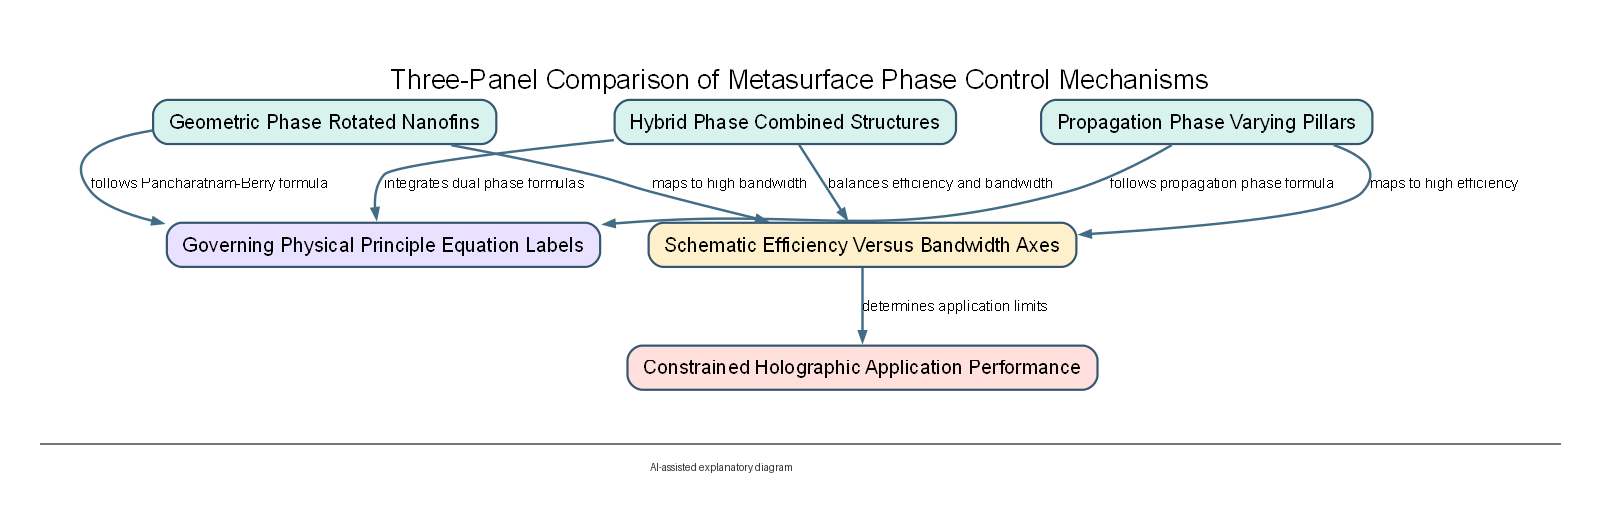
\includegraphics[width=0.9\linewidth,height=\textheight,keepaspectratio,alt={Three-Panel Comparison of Metasurface Phase Control Mechanisms. Distinct phase mechanisms map to specific nanostructures and equations, creating unique efficiency-bandwidth trade-offs that define holographic performance limits. AI-assisted explanatory diagram; not empirical evidence.}]{figures/01_FIG-GEN-001.png}
\caption{Three-Panel Comparison of Metasurface Phase Control Mechanisms. Distinct phase mechanisms map to specific nanostructures and equations, creating unique efficiency-bandwidth trade-offs that define holographic performance limits. AI-assisted explanatory diagram; not empirical evidence.}\label{fig:visual_01}
\end{figure}

Distinct from the geometric phase derived from coordinate rotation, propagation phase relies on optical path length variations and resonant delays within individual meta-atoms to accumulate the necessary wavefront shift. This mechanism often exploits bound states in the continuum (BICs) or Fano resonances to achieve high-quality factor resonances and strong electric field confinement, thereby enabling efficient phase modulation through sharp dispersive spectral features. \citep{doi_10_1002_adpr_202400191_88f03cd9} For instance, hybrid metal-dielectric metasurfaces can support these BICs by restraining radiation loss, where symmetry breaking transforms perfectly localized states into quasi-BICs with tunable quality factors reaching up to 873 for active sensing applications. Similarly, all-dielectric metasurfaces utilize high refractive indices to trap optical modes and generate asymmetric Fano profiles via the interference of localized states with the radiation continuum, offering low dissipative losses compared to metallic counterparts. \citep{doi_10_1021_acsnano_4c16934_9c79f5cf} However, this reliance on resonant spectral features introduces a fundamental constraint: chromatic dispersion. Because the phase response is intrinsically linked to wavelength-dependent resonance conditions, maintaining image quality across the visible spectrum often necessitates complex mitigation strategies, such as dedicating separate waveguide channels to specific RGB colors rather than achieving true single-layer achromaticity. This trade-off between the high efficiency offered by resonant confinement and the limited bandwidth imposed by dispersion underscores the physical boundaries that subsequent hybrid approaches aim to navigate. \citep{doi_10_1002_adpr_202400191_88f03cd9} \citep{s2_42f2fcc893f3a45ac750a8ffe67752f8533c0c61_58d9419c} \citep{doi_10_1038_s41377_025_01761_w_a73a6b84}

Published studies have developed hybrid metal-dielectric metasurfaces that combine metallic and dielectric components to exploit both plasmonic field confinement and low-loss dielectric resonances, aiming to address the efficiency losses inherent in purely plasmonic systems and the dispersion challenges of resonant dielectrics. The optical architecture seeks a balance between strong field enhancement and optical efficiency, often leveraging bound states in the continuum (BICs) to restrain radiation loss while maintaining high quality factors. For instance, hybrid photonic-plasmonic asymmetric gratings have demonstrated the ability to regulate transitions between quasi-BICs and BICs through symmetry breaking in geometry and permittivity, achieving quality factors up to 873 by suppressing radiation loss. In a humidity-modulated strategy, hybrid photonic-plasmonic asymmetric gratings (HPAGs) composed of alternating dielectric gratings on aluminum oxide and gold films utilize polyvinyl alcohol to regulate transitions between quasi-BICs and BICs. As relative humidity increases, the volume expansion and refractive index reduction of the polymer induce symmetry breaking in geometry and permittivity, thereby suppressing radiation loss. \citep{doi_10_1002_adpr_202400191_88f03cd9} Complementing these hybrid strategies, all-dielectric metasurfaces utilizing high-refractive-index materials such as titanium dioxide on quartz or gallium nitride on sapphire substrates offer a pathway to high optical efficiency in the visible spectrum, providing a robust physical basis for phase control compared to metallic alternatives. However, even these advanced systems face boundaries; practical implementations in the near-infrared reveal that residual phase mismatches and fundamental limits on meta-atom transmittance can cap overall system efficiency, suggesting that while hybrid and high-index dielectric approaches mitigate previous trade-offs, they introduce new constraints related to nonlocal behaviors and fabrication tolerances that must be navigated in subsequent design stages. \citep{doi_10_1002_adpr_202400191_88f03cd9} \citep{doi_10_1063_5_0141881_93942631}

The fundamental capacity for wavefront manipulation ultimately rests on the electromagnetic properties of individual meta-atoms, which define the available degrees of freedom for the system, even though hybrid and dielectric strategies offer pathways to balance efficiency and confinement. However, translating desired optical responses into physical geometries is complicated by singular point mutations in the mapping between electromagnetic parameters and structural dimensions, creating non-uniqueness challenges that hinder traditional design approaches. Recent advances address this instability by employing deep residual networks combined with electromagnetic property classification to predict meta-atom geometry from transmission coefficients, effectively mitigating inaccurate predictions caused by these singularities and achieving a mean square error below 0.23 across dataset parameters. \citep{doi_10_1109_iccem60619_2024_10559188_c3199408} \citep{doi_10_1109_isctis58954_2023_10213114_7fee3b45} Complementary frameworks further resolve the many-to-one relationship between design and response spaces by utilizing representation learning to compress high-dimensional data into feature-rich low-dimensional latent spaces, where variational autoencoders coupled with particle swarm optimization can identify global optimal solutions with up to 94\% accuracy. These developments underscore that the intrinsic trade-offs of phase control mechanisms necessitate sophisticated inverse design tools to navigate the complex, non-unique landscape of meta-atom engineering, setting the stage for a broader transition from heuristic methods to automated computational frameworks. \citep{doi_10_1109_iccem60619_2024_10559188_c3199408} \citep{doi_10_2139_ssrn_4082312_28ca582d}

Metasurface engineering has fundamentally transitioned from traditional heuristic approaches to automated inverse design frameworks to navigate the complex trade-offs and non-uniqueness challenges inherent in meta-atom properties. Whereas conventional pattern-to-phase paradigms rely on complex, time-consuming numerical calculations and expert intuition---often limiting the accessible degrees of freedom---modern strategies employ computational methods to directly map desired electromagnetic responses to optimal nanostructure geometries. This shift is exemplified by deep learning architectures that integrate multi-task learning with genetic algorithms, achieving forward prediction accuracies of 96.7\% and inverse design success rates of 83.9\% for silicon nitride disk arrays, thereby overwhelming conventional neural network performance. Similarly, combining deep neural networks with genetic algorithms enables rapid phase-to-pattern mapping, controlling population generation within preset phase ranges to significantly reduce optimization iterations for devices like orbital angular momentum generators and metalenses. Furthermore, novel time-domain inverse design methods using adjustable pulses have emerged to overcome the lengthy simulation times associated with frequency-domain adjoint optimization, facilitating the creation of high-performance metalenses with uniform broadband responses. By replacing laborious brute-forcing processes with these data-driven and algorithmic tools, researchers can now access larger design spaces and more versatile electromagnetic functionalities, directly addressing the physical constraints outlined in previous sections and setting the stage for specific deep learning implementations that learn non-linear input-output relationships. \citep{doi_10_1016_j_rio_2026_100988_b00ee173} \citep{doi_10_1364_oe_478084_bf365dc5} \citep{doi_10_1109_apmc60911_2024_10867828_7c3f3b13}

Deep learning models now address the core challenge of mapping non-linear geometry-response relationships in metasurface inverse design, building on the transition from heuristic to automated frameworks. These models, trained via non-linear activation functions and backpropagation, intelligently learn complex input-output correlations over large datasets, effectively approximating solutions to Maxwell's equations without explicit knowledge of the governing physics. This data-driven approach streamlines the design of bianisotropic and multifunctional metasurfaces by replacing intuitive fine-tuning with surrogate models that rapidly predict unit cell properties. Advanced implementations utilize Gaussian Mixture Models on latent spaces or Generative Adversarial Networks to optimize specific submanifolds, enabling the precise mapping of desired holographic phase profiles to anisotropic meta-atom geometries. However, this framework shift incurs significant upfront computational costs due to the need for extensive, task-specific datasets generated via expensive simulations like FDTD or RCWA, and the resulting performance remains sensitive to dataset quality and hyperparameter optimization. Ultimately, while deep learning expands the accessible design space beyond traditional boundaries, its practical deployment requires careful balancing of data generation expenses against the need for complex, high-fidelity holographic responses. \citep{doi_10_1515_nanoph_2019_0474_d2187501} \citep{doi_10_48550_arxiv_2204_00433_1c5cfd3e} \citep{doi_10_3390_photonics12100947_b44bdefd}

Gradient-based topology optimization offers a rigorous framework for exploring material distributions within simulation domains to discover non-intuitive binary layouts, complementing the strengths of deep learning in mapping non-linear relationships. That implementation treats the design space as a discretized grid where dielectric structures are iteratively updated to maximize a specific figure of merit. Central to this efficiency is adjoint optimization, a method that computes gradients by running just two full-wave simulations per iteration---one forward and one adjoint---regardless of the number of design parameters. To ensure these continuous mathematical solutions translate to feasible fabrication results, researchers employ affine geometric transformations and robustness algorithms that binarize profiles and filter out sub-30 nm features. For instance, such methods have enabled thermal emitters to reach 92\% efficiency through complex freeform geometries that surpass conventional resonators. Furthermore, when combined with neural networks and Fourier-represented loss functions, these inverse design algorithms can rapidly optimize metasurface geometries for high-fidelity wavefront reconstruction, achieving mean squared errors approaching 10\^{}-6 even under noisy conditions. However, while these techniques effectively navigate the trade-offs between efficiency and design flexibility identified earlier, they must still contend with the inherent non-uniqueness of inverse scattering problems, a challenge addressed in the following section. \citep{doi_10_1002_adom_202500249_9967e710} \citep{doi_10_48550_arxiv_2603_15210_fdcfb92f} \citep{doi_10_1515_nanoph_2020_0579_8812c5b1}

Gradient-based and adjoint methods provide efficient pathways to feasible fabrication profiles, yet they operate within a landscape where the inverse design of metasurfaces for holographic wavefront control remains fundamentally ill-posed. This mathematical difficulty arises because determining a physical structure from a desired spectral response involves resolving inherent ambiguities in phase and amplitude coupling, specifically manifesting as a one-to-many mapping where multiple distinct geometric configurations yield identical optical spectra. Such non-uniqueness confuses deterministic optimization algorithms and traditional regression-based neural networks, often leading to mode averaging and the generation of invalid geometries that fail to produce the target spectrum when verified with a Maxwell solver. Furthermore, practical inverse-design problems are frequently under-constrained or evolve dynamically, such as when intelligent metasurfaces face shifting objectives or updated fabrication limits. To mitigate these challenges, representation learning offers a powerful approach by decoupling the search process into input-side models that provide a reusable, physics-agnostic manifold of device geometries and output-side models that act as fast surrogate solvers. \citep{doi_10_2139_ssrn_4082312_28ca582d} This strategy enables efficient exploration and rapid re-optimization of candidates against new targets without the prohibitive computational cost of full-wave electromagnetic simulations at every evaluation step, thereby stabilizing solutions in a design space where global optimization methods would otherwise become computationally infeasible due to exponential scaling. \citep{doi_10_71465_fapm546_bda368a5} \citep{doi_10_1002_adom_202502062_d73a85e1}

The resolution of ill-posed inverse problems has paved the way for advanced algorithms to practically realize multi-channel holography by mapping complex macroscopic targets to microscopic geometries. Deep learning-assisted frameworks address this challenge by decomposing the design space; for instance, specific methodologies employ classifiers to distinguish cross-talk types in dual-spin systems, allowing artificial neural networks to fit non-linear functions between structural parameters and phase responses for quad-channel vortex multiplexing. This data-driven approach extends beyond simple classification to global optimization, where evolutionary algorithms embedded within physical propagation models search for optimal phase masks that satisfy rigorous differential optical field constraints. Furthermore, electromagnetic inverse source methods have been generalized from two-dimensional to three-dimensional configurations, utilizing desired power patterns on perpendicular far-field cuts to infer equivalent surface currents and macroscopic properties. By integrating these computational strategies with the physical degrees of freedom offered by hybrid phase mechanisms, researchers can navigate the non-uniqueness of scattering problems to achieve precise wavefront tailoring across spin, wavelength, and spatial domains, directly addressing the fundamental trade-offs outlined in this chapter. \citep{doi_10_1117_1_apn_2_1_016010_57069347} \citep{doi_10_1117_12_3110717_26d5b63b} \citep{doi_10_1109_lawp_2023_3266337_3b44a88a}

\section{Computational Inverse Design for Metasurface Holograms: From Forward Models to Algorithmic Optimization}\label{computational-inverse-design-for-metasurface-holograms-from-forward-models-to-algorithmic-optimization}

Nanophotonic device design has fundamentally shifted from intuition-based heuristics to rigorous computational inverse design, a transition driven by the need to explore high-dimensional parameter spaces that defy traditional analytical encoding. Inverse design methods utilize effective mathematical approaches to address optimization problems, making them particularly well-suited for achieving complex design targets with extraordinary performance beyond conventional capabilities. This evolution encompasses both classical iterative techniques, such as topology optimization which offers high calculation accuracy at the expense of significant computational consumption, and revolutionary deep learning-based methods that promise to resolve these efficiency bottlenecks. The earliest optimization methods represent the oldest and perhaps most intuitive applications of inverse design, where binary representations and re-parameterization of design structures in topology optimization iterate successive figure-of-merit minimization until reaching an optimal solution. Specifically for metasurface holograms, ODNN research has moved from simple analytical superposition to sophisticated algorithmic strategies like the adjoint gradient method, which calculates gradients of a cost function with respect to all design variables by solving an ``adjoint problem'' with complexity similar to a single forward simulation. \citep{doi_10_48550_arxiv_2603_15210_fdcfb92f} \citep{doi_10_1038_s41598_024_67142_2_db612126} While these advanced approaches enable the parallel optimization of many parameters and facilitate novel architectures like multilayer meta-atoms, they often operate within idealized models that may not fully capture the nonconvex nature of fabrication-induced disorder or the constraints required for physical realizability. Consequently, while modern algorithms theoretically unlock complex wavefront control, their reliance on perfect geometric assumptions creates a critical gap between simulated optimality and the fidelity of real-world fabricated devices. \citep{doi_10_1088_1361_6439_ad3a72_72d60f33} \citep{doi_10_1364_oe_27_030308_704a1c9b} \citep{s2_76a83ea3baed75ad88b7f0782eb9a694a330c853_cee16cac} \citep{doi_10_1515_nanoph_2021_0660_2d91a441}

Inverse design fundamentally reverses the conventional workflow by mapping target electromagnetic performance parameters directly to structural geometries, marking a shift from heuristic intuition to rigorous optimization. While forward design predicts responses from known structures with a straightforward one-to-one relationship, inverse design confronts a mathematically ill-posed challenge where multiple distinct geometric configurations can yield identical optical spectra. This non-uniqueness creates a one-to-many mapping that confuses deterministic algorithms and often leads to mode averaging or invalid geometries in traditional regression models. To address this, modern frameworks employ strategies such as tandem neural networks that couple inverse predictors with fixed forward models, or conditional decoders that integrate Gaussian noise vectors to explore diverse solutions within a latent space. \citep{doi_10_1364_josab_497661_d333080a} \citep{doi_10_1038_s41467_025_57516_z_7c69e056} Furthermore, because purely data-driven approaches may generate structures that appear valid but fail to obey Maxwell's equations, recent advances incorporate physics-informed constraints and spectral priors to ensure generated designs are physically realizable. Despite these algorithmic sophistication, the reliance on idealized mappings highlights the fragility of current methods when facing the complex, non-linear resonance modes of real-world fabrication, setting the stage for gradient-based techniques that attempt to navigate these continuous parameter spaces more robustly. \citep{doi_10_1088_1361_6463_ad3e05_d24e0a0a} \citep{doi_10_23919_piers_fall62445_2025_11394631_4fdb8517} \citep{doi_10_71465_fapm546_bda368a5}

Gradient-based topology optimization serves as an iterative strategy for navigating the expansive design spaces inherent in inverse problem formulations, aiming to optimize material distribution within a simulation domain to meet specific optical objectives. Central to the same strategy is the adjoint method, a technique that efficiently calculates gradient information required for design updates using only two full-wave simulations---one forward and one adjoint---regardless of the number of design parameters. \citep{doi_10_1088_1367_2630_acfcd6_32444f17} This efficiency allows for the exploration of complex, non-intuitive geometries in broadband regimes with arbitrary dispersive materials, far surpassing the capabilities of parametric sweeps or stochastic methods like genetic algorithms which struggle with high-dimensional spaces. For instance, applying this method to thermal emitters has yielded freeform binary layouts with efficiencies reaching 92\%, significantly outperforming conventional resonator designs. Adjoint-based topology optimization has been applied to the inverse design of sub-diffraction focusing metalenses, enabling the generation of complex geometries that surpass conventional diffraction limits. \citep{doi_10_1088_1367_2630_acfcd6_32444f17} However, a critical disconnect emerges between these algorithmic successes and physical realization: while the optimization often operates on continuous profiles or intermediate density values to facilitate smooth convergence, the final output must undergo a binarization process to become fabrication-feasible. This post-processing step, which forces continuous variables into discrete material states, can introduce performance deviations and increases computational complexity when repeated iteratively, underscoring the tension between idealized continuous optimization and the discrete constraints of nanofabrication. \citep{doi_10_48550_arxiv_2603_15210_fdcfb92f} \citep{doi_10_1021_acsphotonics_3c00572_fda8f742} \citep{doi_10_1002_adom_202500249_9967e710}

The integration of deep learning into continuous parameter optimization frameworks has triggered a paradigm shift by employing fully connected neural networks to approximate forward scattering functions, thus supplanting computationally expensive electromagnetic solvers. This design relies on a surrogate model, defined here as a neural network trained to generate accurate electromagnetic responses from geometric topologies without running iterative simulations. \citep{doi_10_1109_jmmct_2025_3544270_6b4eb6dd} By learning these mappings, machine learning approaches address the computational resource and time constraints of conventional design methods, enabling efficient, rapid design on demand where structures are computed directly from desired targets. For instance, physics-based neural network surrogate models have been combined with optimization algorithms to search phase libraries for specific applications, such as designing orbital angular momentum multiplexers that successfully transmitted high-speed signals. Neural network-based surrogate models have been developed for the inverse design of metasurfaces, offering a rapid alternative to slow electromagnetic solvers by learning the mapping between structural parameters and optical responses. \citep{doi_10_1364_prj_450564_4b46735d} While this strategy effectively bypasses the prohibitive costs of massive electromagnetic iterations required by traditional parameter sweeps, it represents a transition from rigorous physical solving to data-driven approximation, setting the stage for specialized architectures needed to resolve the inherent non-uniqueness of mapping optical responses back to geometry. \citep{doi_10_71465_fapm546_bda368a5} \citep{doi_10_1364_prj_450564_4b46735d} \citep{doi_10_1088_1361_6463_ab8036_d433363a}

Standard surrogate models accelerate design but often struggle with the non-uniqueness inherent in mapping optical responses back to geometry, a challenge addressed by advanced tandem and cascaded architectures. A tandem network typically pairs an inverse predictor with a forward model to resolve ambiguities, ensuring that generated structures yield the desired optical output. Extending this concept, cascaded neural network architectures comprise separate forward and inverse design networks that enable cyclical optimization for targeted nanophotonic functionalities, effectively addressing the complexity of simultaneous problem solving. For instance, specific implementations utilize deep residual networks combined with electromagnetic property classification to predict meta-atom geometry from transmission coefficients, a method that mitigates errors caused by singular point mutations in the mapping process and achieves a mean square error of less than 0.23. Deep neural networks integrating multi-task learning with genetic algorithms have been utilized for the forward prediction and inverse design of metasurfaces, allowing for the accurate determination of meta-atom geometries from desired transmission coefficients. \citep{doi_10_1016_j_rio_2026_100988_b00ee173} Similarly, cyclical frameworks have been proposed where a generative model creates structural designs while a simulation neural network evaluates their authenticity, guiding the discovery of metasurfaces without strict structural restrictions. However, these sophisticated approaches are not without limitations; cascaded methods may still force convergence to only one of several valid solutions, and simultaneous training can introduce hyper-parameter dependencies that hinder proper convergence. Thus, while these advanced topologies significantly refine the theoretical fidelity of hologram generation, they operate within constrained solution spaces that foreshadow the broader generalization challenges discussed next. \citep{doi_10_1038_s41598_020_76400_y_aa62c15d} \citep{doi_10_1109_iccem60619_2024_10559188_c3199408}

A fundamental constraint persists despite the use of advanced network architectures like tandem and cascaded models to address non-uniqueness in hologram generation: neural networks trained for inverse design cannot generalize effectively beyond the specific information distributions present in their training datasets. This limitation necessitates hybrid algorithms that combine data-driven approaches with conventional optimization strategies to mitigate performance gaps outside the training domain. In such hybrid frameworks, the neural network performs a rough global search to estimate a desired solution, while an iterative optimization algorithm, such as the adjoint method, executes a local refinement step to push performance further, thereby overcoming the individual restrictions of both techniques. To specifically address the challenge of applying these models across distinct functionalities without retraining from scratch, transfer learning has emerged as a critical enabler. By fine-tuning specific inverse design network parameters while freezing the hidden layers, this method allows knowledge to be transferred between heterogeneous metasurface datasets, such as moving from electromagnetic-induced transparency domains to absorption or phase-controlled targets. \citep{doi_10_1364_ol_514212_108a4a7f} \citep{doi_10_1109_ieeeconf35879_2020_9330480_27bef614} Remarkably, the proposed network can complete training processes with as few as 700 target domain samples, significantly lowering the data threshold required for cross-domain design. These hybrid and transfer learning strategies represent essential steps toward robust inverse design, yet they still operate within simulated environments that often ignore the stochastic realities of fabrication, a disconnect that ultimately limits the fidelity of realized devices. \citep{doi_10_1021_acsphotonics_2c00968_06a2e96b} \citep{doi_10_1364_ol_514212_108a4a7f}

Inverse design methods now actively exploit high degrees of freedom in metasurface geometry to manipulate light-matter interactions beyond simple phase control, building on hybrid strategies that mitigate generalization limits. The configuration moves past intuition-based heuristics by treating complex structural parameters as optimizable variables. For instance, optical multilayer thin film structures, which consist of multiple stacked layers with thicknesses ranging from tens to hundreds of nanometers, present a combinatorial optimization problem where determining the best material combination and thickness for desired responses lacks a closed-form solution. Modern algorithms address this by automatically identifying optimal structures, while deep learning models can establish direct mappings from optical responses to geometric configurations, completing designs in fractions of a second compared to traditional optimization. These techniques enable specific functional applications, such as using inverse-designed dielectric metasurfaces for arbitrary-angle image relay with aberration correction, where neural networks optimize phase responses to compensate for severe distortions in deflected images. Furthermore, deep learning facilitates the inverse design of reflective metasurface antennas by leveraging small-scale statistically random data selection to map unit cell statistics to full-array configurations, thereby bypassing exhaustive parametric sweeps. Extending these capabilities to larger scales, fast direct solvers now enable the full-wave inverse design of centimeter-scale cylindrical metasurfaces, allowing computational optimization of large-area holographic elements that were previously intractable due to simulation cost. By unlocking these complex geometries, computational tools transform theoretical versatility into tangible device architectures, though this reliance on precise geometric definition sets the stage for examining how fabrication imperfections challenge these idealized models. \citep{doi_10_1016_j_isci_2025_112222_1f7c10f5} \citep{doi_10_1364_oe_519179_39046c11} \citep{doi_10_1002_mop_34068_b2e55b41} \citep{doi_10_1515_nanoph_2024_0127_c4fd5a12}

Despite the advanced capabilities of inverse design algorithms to exploit high-dimensional degrees of freedom, a critical design-reality gap emerges from their reliance on idealized models that assume precise geometric control. Optimization strategies frequently depend on symmetry-breaking perturbations or quasi-bound states in the continuum (quasi-BIC), where optical lifetimes are tuned by adjusting perturbation strength under the assumption of perfect fabrication. However, heuristic optimization methods often produce target phase profiles or transfer matrices that are not physically realizable; when these idealized designs are projected onto feasible metasurface structures, the mismatch leads to significant deviations in optical behavior and degraded performance. Efforts to mitigate this issue, such as applying smoothness regularization to phase profiles to ease hardware design, have generally been inadequate because while smoother profiles are simpler to implement, they significantly limit expressivity and do not ensure true physical feasibility. Similarly, physics-informed machine learning models for optical metamaterials often minimize only the optical reconstruction cost function while lacking explicit constraints on design parameters in the loss function, potentially yielding solutions far from ground truth or practical feasibility. While techniques like simulation-in-the-loop training attempt to enforce physical constraints via adjoint methods, they remain prohibitively expensive for large-scale systems, leaving many optimized designs vulnerable to fabrication-induced disorder. This disconnect underscores the chapter's central thesis: without integrating realistic fabrication constraints directly into the optimization objective, sophisticated algorithms will continue to produce theoretically optimal but practically fragile devices. \citep{doi_10_1103_physrevapplied_21_044004_d1b93ffe} \citep{doi_10_48550_arxiv_2505_18377_a6fc9ec3} \citep{doi_10_1002_adpr_202300158_66d61883}

\section{Nanofabrication of Metasurface Holograms: Tolerances, Disorder, and Scalability}\label{nanofabrication-of-metasurface-holograms-tolerances-disorder-and-scalability}

Inverse design methods, including deep learning and optimization algorithms, are increasingly utilized to address the high-dimensional parameter spaces inherent in nanophotonic metasurface hologram fabrication, effectively overcoming the limitations of traditional intuition-based approaches. \citep{doi_10_1109_metamaterials54993_2022_9920895_1a67346a} These methodologies generate complex continuous or discrete geometric profiles that often require binarization and discretization steps to become physically fabricable, creating an immediate dependency on high-precision nanofabrication techniques such as electron-beam lithography to realize the proposed structures. While classical iterative methods offer high calculation accuracy, they face significant challenges regarding computational consumption when addressing multi-objective or multi-scale design requirements, prompting a shift toward deep learning strategies that promise greater efficiency in exploring vast design spaces. However, the transition from these sophisticated computational models to physical devices introduces a critical bottleneck: the intricate geometries produced by adjoint-based gradient evaluation and neural networks demand fabrication tolerances that push the limits of current manufacturing capabilities, setting the stage for an analysis of the specific research-scale tools currently employed to meet these demands. \citep{doi_10_1088_1361_6439_ad3a72_72d60f33} \citep{doi_10_48550_arxiv_2603_15210_fdcfb92f} \citep{doi_10_1109_metamaterials54993_2022_9920895_1a67346a}

Current research predominantly relies on high-precision nanofabrication technologies capable of engineering light-matter interactions at the nanoscale to realize the complex geometric profiles generated by inverse design algorithms. Specifically, metasurface holograms are typically fabricated using techniques such as focused ion-beam milling and various lithographic methods, which enable the manufacturing of structures with features near or below the electromagnetic wavelength. For instance, a monolithic lithium niobate (LiNbO3) metasurface operating in the visible range was realized through ion beam milling to overcome nanofabrication challenges that typically limit nanostructure aspect ratios and minimum sizes. \citep{doi_10_1021_acsphotonics_1c00026_bdd15a92} Among these, electron-beam lithography (EBL) serves as a standard research-scale tool, operating as a serial writing technique that directs a focused beam of electrons to pattern substrates with exceptional resolution. \citep{doi_10_1088_1361_6528_ad3c4c_ac8a5241} \citep{doi_10_1021_acsomega_4c01044_0ad8ee05} While these advances have made possible compact optical systems with new functionalities like beam steering and light structuring, the very mechanism that ensures high fidelity---serial processing---imposes a critical bottleneck. Because these methods write patterns point-by-point or feature-by-feature rather than in parallel, they suffer from inherently low throughput, restricting production to small-scale demonstrations. This reliance on serial fabrication creates an immediate tension: while computational methods can explore practically unlimited design spaces to optimize performance, the physical realization of these innovative designs remains constrained by the slow speed of current manufacturing processes, thereby hindering the transition from laboratory concepts to scalable applications. \citep{doi_10_1021_acsphotonics_3c00572_fda8f742} \citep{doi_10_1002_inf2_12116_b5c46838}

High-resolution serial writing techniques enable the initial prototyping of complex profiles, yet the translation from computational inverse design to physical metasurface structures inevitably introduces structural disorder, defined here as deviations including sidewall angles, feature roughness, and placement errors that systematically degrade optical performance. This degradation is particularly acute in machine-learning and optimization-based approaches, where constituent unit cells are granted the flexibility to adopt completely different primitives from their neighbors to match desired surface parameters. Although this geometric diversity is necessary for achieving specific electromagnetic responses, it creates significant fabrication challenges; the abrupt changes in physical structure across the surface can lead to unpredictable levels of additional mutual coupling that are not captured in homogenized design models. Evidence suggests that while such methods can successfully guide the inverse design of nonuniform metasurfaces, the resulting discrepancies often manifest as errors in null realization and sidelobe levels in the far-field radiation pattern. Furthermore, advanced strategies employing adjoint-based gradient evaluation with affine geometric transformations allow for the simultaneous optimization of orientation, position, and size, yet the requirement to binarize these continuous profiles for feasible fabrication adds computational complexity and potential fidelity loss. Consequently, the very geometric freedom that empowers modern inverse design algorithms becomes a source of uncertainty during physical realization, driving a wedge between theoretical predictions and experimental holographic fidelity. \citep{doi_10_48550_arxiv_2603_15210_fdcfb92f} \citep{doi_10_1109_tap_2021_3137496_d4a1d597}

A more fundamental barrier exists beyond the structural disorder introduced during physical realization: the algorithms themselves often propose designs that are inherently unrealizable. Inverse design methods for photonic metasurfaces frequently generate target phase profiles or transfer matrices that cannot be physically constructed due to strict fabrication constraints. When these idealized, abstract models are projected onto feasible metasurface structures, the resulting mismatch causes significant deviations in optical behavior and degraded performance. While heuristic approaches have attempted to mitigate this by applying smoothness regularization to ease hardware design, such measures are generally inadequate; they limit the system's expressivity without ensuring true physical feasibility, often still yielding impractical designs. Conversely, simulation-in-the-loop training enforces feasibility by embedding optimization directly within the training loop using adjoint methods, yet the resulting design remains prohibitively expensive and unscalable for large systems because it requires solving Maxwell's equations at every iteration. This persistent disconnect between computational output and physical reality underscores the critical gap where algorithmic potential is stifled by the lack of scalable, physics-aware optimization schemes. \citep{doi_10_48550_arxiv_2505_18377_a6fc9ec3}

Scalable manufacturing strategies such as nanoimprint lithography (NIL) have been proposed as primary candidates for mass production to address the throughput bottlenecks inherent in serial lithography methods. NIL operates on an intuitive mechanical principle where a master mold containing the inverse nanopattern is pressed into a resist material, allowing for the parallel replication of complex metasurface geometries rather than writing them point-by-point. \citep{doi_10_3390_encyclopedia5040197_fe6bfdc9} \citep{doi_10_5772_intechopen_72534_9965e900} The optical architecture theoretically offers a pathway to overcome the significant increases in manufacturing difficulty and cost associated with the integrated characteristics of metasurfaces, particularly for applications demanding ultra-miniaturization and high-quality light field modulation like future 3D displays. Evidence suggests that while materials like TiO2 can improve work efficiency, their preparation via atomic layer deposition remains time-prohibitive for commercialization, underscoring the urgent need for more efficient micro-nano processing methods to solve these production problems. However, despite the promise of NIL and roll-to-roll processing to enable lighter weight systems with larger fields of view, the ability of these techniques to maintain the nanometer-scale fidelity required for high-efficiency holographic reconstruction remains largely unvalidated at meter-scale areas, leaving a critical gap between proposed scalable solutions and the rigorous demands of ultimate commercialization. \citep{doi_10_1515_nanoph_2025_0269_b999ce93}

Scalable pathways such as nanoimprint lithography theoretically enable meter-scale production, yet the current scientific record reveals a critical validation deficit: evidence heavily favors computational design methodologies over experimental verification of these manufacturing processes at scale. Recent advances demonstrate sophisticated deep learning-driven frameworks, including convolutional neural networks and generative adversarial networks, which successfully optimize metasurface unit modes and capture target features for holographic imaging. For instance, deep convolutional generative adversarial networks have been employed to inversely design electromagnetically induced transparency metasurfaces, demonstrating the capability of such frameworks to optimize unit modes and capture target features for holographic imaging. \citep{doi_10_1088_1402_4896_acf007_ad71688e} Similarly, large-scale photonic inverse design has progressed through adjoint optimization and topology optimization techniques capable of addressing centimeter-scale cylindrical metasurfaces. Advances in this area include the use of multi-objective optimization aided inverse-design methods for metasurface synthesis, illustrating how computational techniques are being applied to address complex photonic design challenges. \citep{doi_10_1117_12_2529823_81c5e659} However, these developments remain predominantly confined to the computational domain, focusing on algorithmic efficiency and latent space exploration rather than the physical tolerances required for industrial replication. Consequently, despite the maturity of design tools that can theoretically generate complex freeform patterns, there is a lack of experimental data confirming that scalable methods can maintain nanometer-scale fidelity when transitioning from simulation to meter-scale fabrication. This disconnect reinforces the chapter's central thesis that the bottleneck in metasurface holography has shifted from design capability to the unvalidated reality of scalable manufacturing, leaving the fidelity of large-area devices as an open and critical challenge. \citep{doi_10_3390_photonics12100947_b44bdefd} \citep{doi_10_1515_nanoph_2024_0127_c4fd5a12}

\section{Active Modulation Mechanisms for Dynamic Metasurface Holography: Speed, Efficiency, and Spectral Trade-offs}\label{active-modulation-mechanisms-for-dynamic-metasurface-holography-speed-efficiency-and-spectral-trade-offs}

Conventional metasurfaces function as static devices, meaning their optical capabilities are permanently fixed at the moment of fabrication. This intrinsic ``write-once'' characteristic creates a fundamental operational ceiling: while these nanostructured surfaces offer powerful wavefront shaping, they lack the adaptability required for dynamic scenarios such as real-time holographic displays. \citep{doi_10_1002_lpor_71186_5fa1be75} Although research efforts have attempted to overcome this rigidity by integrating active materials or mechanical displacement systems, these modifications often introduce significant penalties, including high optical loss, increased fabrication complexity, or reliance on bulky actuators that compromise the miniature form factor. Consequently, the inability of standard metasurfaces to reconfigure their phase profiles post-fabrication necessitates the exploration of specialized active modulation mechanisms. Addressing this limitation is critical to resolving the speed-efficiency-bandwidth trilemma, as the transition from static to dynamic operation defines the primary challenge in developing practical, reconfigurable holographic systems. \citep{doi_10_1002_nap2_70185_56c8ab30}

Phase-change materials (PCMs) offer a pathway to non-volatile reconfiguration by altering the refractive index through structural phase transitions, thereby overcoming the static limitations of conventional metasurfaces. \citep{doi_10_1515_nanoph_2024_0357_805aeaf6} In dynamic nonlocal metasurfaces, this mechanism enables multifunctional integration by modifying meta-atom parameters, such as rotation angles, to achieve tunable optical responses without redesigning the entire lattice. Representative evidence demonstrates this using vanadium dioxide (VO2), where increasing ambient temperature from 30 \(^\circ\) C to 53 \(^\circ\) C shifts the device from an insulator state to a dynamic metalens capable of narrow-band focusing. For instance, a MoS2/VO2/Au/Si metasurface was developed to dynamically tune optical absorbance and structural color by leveraging the temperature-dependent dielectric response of VO2. Heating this device induces an insulating-to-metallic transition that alters the O-2p state transitions, enabling active control over its optical properties. \citep{doi_10_1515_nanoph_2023_0169_6ba026c6} The working frequency becomes tunable as the converted right-circularly polarized light dynamically focuses around different resonances corresponding to these temperature changes. However, this thermal modulation incurs a distinct penalty: the transmission intensity of the focused light gradually decreases with rising temperature due to increased inherent material losses. Consequently, while PCMs provide robust spectral control determined by engineering a single meta-atom, they introduce a trade-off between tunability and diffraction efficiency driven by absorption, setting the stage for alternative continuous tuning methods that may mitigate these loss mechanisms. \citep{doi_10_1515_nanoph_2024_0357_805aeaf6}

Figure \ref{fig:visual_02} shows Position active modulation platforms (phase-change materials, liquid crystals, MEMS actuators, graphene, electro-optic polymers) on a speed-efficiency-bandwidth performance triangle, illustrating the fundamental trilemma\ldots{}

\begin{figure}
\centering
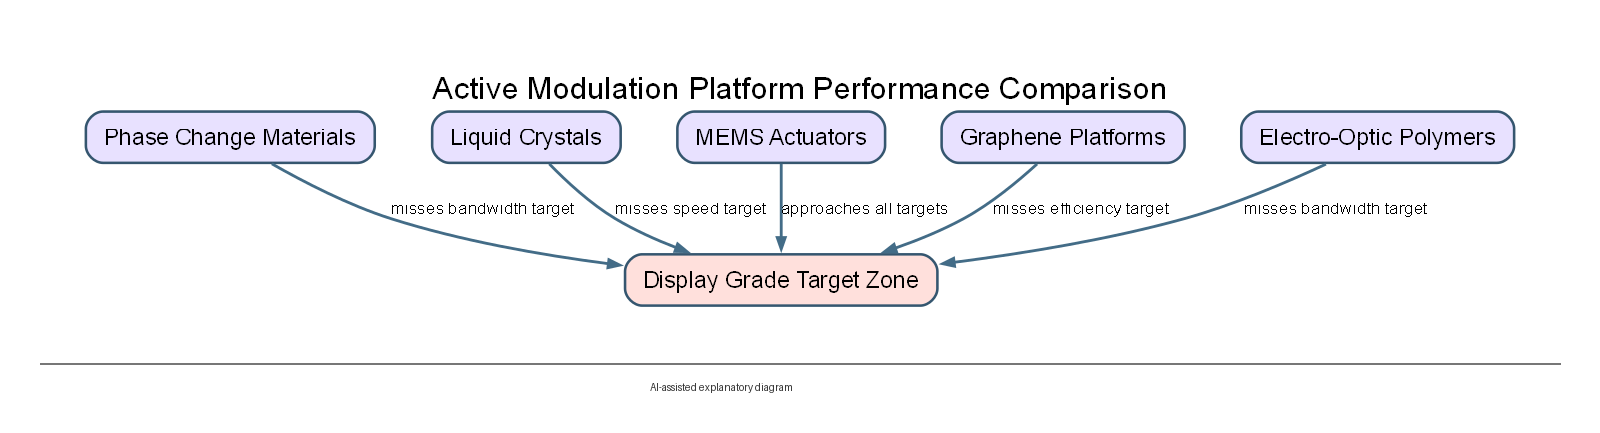
\includegraphics[width=0.9\linewidth,height=\textheight,keepaspectratio,alt={Active Modulation Platform Performance Comparison. No single active modulation platform currently satisfies the simultaneous speed, efficiency, and bandwidth requirements of the display-grade target zone. AI-assisted explanatory diagram; not empirical evidence.}]{figures/02_FIG-GEN-002.png}
\caption{Active Modulation Platform Performance Comparison. No single active modulation platform currently satisfies the simultaneous speed, efficiency, and bandwidth requirements of the display-grade target zone. AI-assisted explanatory diagram; not empirical evidence.}\label{fig:visual_02}
\end{figure}

Hybrid meta-optic systems offer an alternative pathway to high-performance operation by combining metasurfaces with refractive optics to achieve continuous analog control, providing a distinct approach from the non-volatile switching enabled by phase-change materials. In this architecture, conventional refractive elements provide the primary optical power, while integrated metasurfaces function as correctors to mitigate aberrations such as coma and chromatic distortion that typically limit pure flat optics. This synergistic mechanism enables large spatial-spectral bandwidth performance, effectively addressing the trade-offs that hinder conventional multi-lens assemblies in applications like long-wave infrared thermal imaging. Representative implementations demonstrate that interleaving metasurface and refractive components can elevate average focusing efficiency from approximately 38\% to over 90\%, while simultaneously achieving wide fields of view exceeding 120 \(^\circ\) across broad spectral bands. Although these hybrid designs significantly enhance system compactness and support real-time vision tasks in augmented reality, they illustrate that overcoming bandwidth limitations often requires complex integration rather than relying on a single active material layer, reinforcing the chapter's thesis that distinct architectural compromises remain necessary to balance speed, efficiency, and spectral range. \citep{doi_10_1002_lpor_71431_d57da40c} \citep{doi_10_1364_ao_516890_6221deea}

Moving beyond the continuous but spectrally restricted tuning of liquid crystals, elastically reconfigurable metasurfaces offer a distinct mechanical pathway to dynamic holography by physically altering meta-atom geometry to achieve large phase shifts. These systems operate on the intuitive principle that simultaneously modulating a structure's effective mass and stiffness can control wave propagation while maintaining impedance matching for high transmission. Traditional design approaches relying on parameter sweeps or topological optimization often struggle with the computational burden of balancing these multi-dimensional variables, particularly when targeting multifunctional performance. However, recent advances demonstrate that data-driven machine learning can serve as a powerful tool to build the necessary nonlinear mappings between high-dimensional inputs and outputs, enabling the inverse design of elements that cover a full 2 \(\pi\) phase shift span without sacrificing transmission efficiency. Complementing these general machine learning strategies, spatial coupled mode theory combined with differentiable neural simulators has emerged as a specific framework for computationally efficient optimization of metasurface geometries for spectral imaging and holographic applications. By replacing traditional electromagnetic solvers with efficient approximations, that implementation enables joint optimization of optical encoders and reconstruction networks, achieving order-of-magnitude reductions in design cycle time compared to full-wave simulations. While this mechanical approach successfully decouples phase control from absorption losses common in electronic methods, it inherently introduces the speed constraints associated with physical actuation, reinforcing the chapter's central thesis that achieving dynamic reconfiguration inevitably requires navigating trade-offs between modulation depth, efficiency, and response time. \citep{doi_10_1016_j_matdes_2022_111560_e69e3350} \citep{doi_10_1021_acsphotonics_4c00171_f68cb79c} \citep{s2_76a83ea3baed75ad88b7f0782eb9a694a330c853_cee16cac}

Transitioning from the mechanical limits of MEMS, electronic modulation via metalenses offers a pathway to ultrafast switching by manipulating light fields through subwavelength micro- and nanostructures. These devices provide a lightweight and easily integrable platform that supports multidimensional wavefront control, enabling innovations in computational-generated holography and near-eye displays. Thermally-modulated Nanophotonic Phased Arrays (NPAs) have been developed as holographic displays that integrate light sources and offer higher refresh rates compared to other technologies. To address the thermal proximity effect, where heating one pixel affects the temperature of nearby pixels, proximity effect correction methods have been extended to Fresnel holograms with phase-only optimization. \citep{doi_10_1109_vr50410_2021_00058_601721f7} Unlike mechanical actuators, metalenses rely on static structural geometry or carrier dynamics rather than physical movement, theoretically allowing for rapid reconfiguration. However, while the same strategy excels in integration and form factor, it faces stringent constraints regarding spectral bandwidth. Current fabrication frameworks limit the magnitude of phase dispersion achievable by individual meta-atoms, creating a mutual trade-off between aperture size, numerical aperture, and operational bandwidth. Consequently, strict achromatism across continuous spectra remains nearly unattainable for large-aperture devices, forcing designers to accept non-strictly achromatic performance or reduced apertures. This highlights a critical efficiency-bandwidth penalty: while electronic and structural modulation solves the speed bottleneck inherent in mechanical systems, it introduces new limitations in spectral range and scalability that prevent a universal solution. \citep{doi_10_1038_s41377_026_02272_y_42e58df2}

Metasurfaces provide unprecedented control over light properties such as amplitude, phase, and polarization to generate high-quality holograms and structural colors for 3D displays. Synthesizing the performance of active modulation platforms reveals a fundamental bottleneck: the speed-efficiency-bandwidth trilemma. Although these planar optics offer high degrees of freedom in designing spatial inhomogeneity over optically thin surfaces, achieving ultimate commercialization requires frame rates approaching infinity, a target that remains distant as current solutions like orbital angular momentum multiplexing only partially address dynamic needs. The evidence indicates that critical parameters are mutually restricted; specifically, the numerical aperture, efficiency, and working bandwidth of achromatic metalenses cannot be simultaneously optimized, and increasing design complexity often introduces crosstalk that degrades work efficiency. Furthermore, material selection presents conflicting constraints where low-loss materials like TiO2 improve efficiency but suffer from time-consuming fabrication, while silicon alternatives offer different trade-offs with lower diffraction efficiency. Consequently, no single active mechanism currently dominates all three axes, confirming that practical dynamic holographic displays must navigate inherent compromises between switching speed, optical efficiency, and spectral range rather than expecting a universal solution. \citep{doi_10_1515_nanoph_2025_0269_b999ce93} \citep{doi_10_1002_inf2_12116_b5c46838}

\section{Metasurface-Integrated Imaging Systems and Optical Computing: Beyond Display Applications}\label{metasurface-integrated-imaging-systems-and-optical-computing-beyond-display-applications}

Inverse design, an optimization process that determines nanostructure geometry directly from a desired optical response, serves as the key mechanism for transitioning metasurface holography from static display patterns to dynamic computational imaging. \citep{doi_10_48550_arxiv_2506_21748_dc49c062} \citep{doi_10_1117_12_3099014_831c7349} Unlike conventional forward modeling, which simulates the output of a fixed structure, inverse design navigates high-dimensional parameter spaces to achieve complex, multi-objective targets that exceed conventional capabilities. Traditional approaches utilize iterative methods, such as topology optimization or evolutionary algorithms, which offer high calculation accuracy but often suffer from excessive computational consumption when addressing multi-scale or multi-physics challenges. To overcome these efficiency bottlenecks, data-driven machine learning methods have emerged as revolutionary alternatives, employing deep neural networks to build surrogate models that provide fast predictions and bypass slow, iterative electromagnetic solvers. These frameworks enable the streamlined creation of complex metasurfaces by mapping target optical responses directly to nanophotonic geometries, effectively addressing the growing conflict between design complexity and limited computing resources. While classical methods remain valuable for specific precision tasks, the integration of deep learning is essential for realizing the sophisticated, aberration-compensated systems required for advanced non-display applications. \citep{doi_10_1088_1361_6439_ad3a72_72d60f33} \citep{doi_10_48550_arxiv_2204_00433_1c5cfd3e}

Hybrid algorithms now combine neural networks with traditional optimization to improve generalization beyond specific training distributions, addressing the foundational need for inverse design. While purely data-driven frameworks predict structural topologies, they often struggle with varying material properties or out-of-plane parameters, necessitating a unified approach that embeds physical constraints directly into the learning process. Physics-informed machine learning addresses this by integrating governing equations, such as Maxwell's wave equations, into loss functions or network architectures to act as regularizers. \citep{doi_10_21070_acopen_10_2025_12939_5a404b4e} \citep{doi_10_1109_tmtt_2026_3658422_94a01e71} This mechanism penalizes predictions violating conservation laws or symmetry requirements, effectively reducing the search space and allowing models to achieve high accuracy with less labeled data while maintaining interpretability. \citep{doi_10_71465_fapm546_bda368a5} Furthermore, because the inverse design problem is mathematically ill-posed due to one-to-many mappings where distinct geometries yield identical spectra, physics-informed diffusion models have been introduced to incorporate spectral constraints. These models ensure that generated designs obey fundamental electromagnetic laws, thereby closing the simulation-reality gap where geometrically valid structures might otherwise fail to produce target optical responses. By coupling physical priors with generative capabilities, these advanced strategies overcome the limitations of black-box deep learning, directly enabling the robust designs required to correct aberrations in practical metalens imaging systems. \citep{doi_10_1002_adom_202100548_6789fa4c} \citep{doi_10_1002_adpr_202300158_66d61883} \citep{doi_10_71465_fapm546_bda368a5}

Transitioning from these robust physics-informed design strategies to their practical deployment, metalens-based imaging systems now utilize computational reconstruction to actively compensate for inherent metasurface aberrations. This shift enables high-resolution miniaturized microscopy and compact, stable three-dimensional tomography without moving parts, surpassing the capabilities of passive optical elements alone. While metalenses offer unique advantages through customized meta-atoms for compact light manipulation, achieving strict achromatism via phase matching remains nearly unattainable for apertures exceeding ten-thousand wavelengths due to fundamental fabrication constraints. To address this, computational inverse design frameworks optimize cascaded metasurface systems by evaluating output intensity and cost functions using angular spectrum wave propagators, which avoid the paraxial approximations of traditional Fresnel diffraction integrals. \citep{doi_10_1364_oe_448757_33bdf93c} \citep{doi_10_1002_lpor_202401011_3926c17d} This design allows for the mitigation of chromatic aberration through structural design rather than relying solely on dispersion engineering, facilitating monolithic integration that yields minimalist optical systems capable of achromatic imaging within an extended field of view. Furthermore, these multi-element cascaded configurations, such as triplets, extend beyond simple correction to characterize complex three-dimensional optical intensity distributions, demonstrating the capability of such systems for advanced wavefront shaping in computational imaging. By shifting the burden of correction from purely geometric nanostructure design to a co-design of optics and algorithms, these systems resolve the trade-offs between aperture size, numerical aperture, and operational bandwidth, directly advancing the chapter's thesis that distinct application domains require tailored strategies coupling physical mechanisms with algorithmic reconstruction. \citep{doi_10_3788_pi_2023_c01_9f71817a} \citep{doi_10_1364_oe_27_030308_704a1c9b} \citep{doi_10_1038_s41377_026_02272_y_42e58df2}

Specialized applications now leverage end-to-end co-design to directly map physical quantities rather than merely forming visual images, building on the computational correction of aberrations in standard metalens imaging. In parallel coded ptychography, a disorder-engineered surface integrating phase scatters and intensity absorbers addresses the scaling complexity obstacles that impede large-scale array microscopy. This turnkey system achieves an imaging throughput orders of magnitude higher than previous implementations by permanently attaching the engineered facet to the image sensor, thereby eliminating mechanical stability issues and enabling open-loop optical acquisition without precise scanning. Similarly, end-to-end co-design of metasurface optics and nonlinear regression algorithms enables broadband temperature imaging by directly mapping thermal radiation spectra to spatial temperature distributions. In a 2024 study, researchers demonstrated end-to-end co-design of a single-layer metasurface frontend with a nonlinear `Planck regression' backend to map broadband thermal radiation spectra directly to spatial temperature distributions. The proposed network optimized the manufacturable metasurface alongside the reconstruction algorithm to handle severe chromatic aberration, yielding high-quality, noise-robust reconstructions of arbitrary temperature maps from long-wavelength infrared data in simulations. \citep{doi_10_1002_adom_202402498_4083d234} The configuration utilizes a ``Planck regression'' algorithm that exploits blackbody radiation physics as a strong prior to infer temperature maps from grayscale long-wavelength infrared images. Unlike conventional thermal systems requiring bulky achromatic optics or complex multi-layer fabrication, this synergistic combination of a single-layer metasurface and computational reconstruction bypasses fundamental delay-bandwidth constraints. Crucially, the metasurface alone does not produce a usable image; meaningful reconstruction emerges only from the joint optimization of the optical encoding and the physics-informed decoder. These high-value applications illustrate how tailored inverse design strategies couple specific physical mechanisms with algorithmic reconstruction to meet the unique constraints of biomedical imaging and thermography. \citep{doi_10_1021_acsphotonics_1c01085_479fdea3} \citep{doi_10_1002_adom_202402498_4083d234}

Deep-learning-assisted inverse design now enables independent control over multiple degrees of freedom, such as spin and frequency, to achieve complex multi-channel holographic tasks. The resulting design addresses the challenge of crosstalk by employing a hybrid methodology where a classifier first distinguishes specific phase modulation requirements, allowing pretrained artificial neural networks to fit the nonlinear functions between physical parameters and propagation phases under distinct conditions. For instance, this framework facilitates the creation of dual-spin and dual-frequency metasurfaces capable of quad-channel off-axis vortex multiplexing, where high-frequency parameters are determined first and serve as preset conditions for the adaptive optimization of low-frequency parameters. Complementing this data-driven strategy, nonlocal Huygens' meta-lenses offer a physics-based route to high-quality-factor spin-multiplexed imaging by decoupling phase and amplitude responses, thereby enabling independent manipulation of orthogonal circular polarizations essential for combining bright-field and edge-enhanced imaging without spectral crosstalk. These advances, ranging from generative adversarial networks learning complex mappings to latent space optimization, collectively demonstrate how algorithmic reconstruction and tailored inverse design overcome the limitations of traditional manual processes, directly supporting the chapter's thesis that distinct application domains require coupled physical and algorithmic solutions to manage resolution and channel count. \citep{doi_10_1117_1_apn_2_1_016010_57069347} \citep{doi_10_1038_s41377_024_01728_3_7dbdfab0} \citep{doi_10_3390_photonics12100947_b44bdefd}

Metasurfaces can be reconfigured to perform mathematical operations directly through light propagation, a paradigm known as optical computing, building on the multi-channel control established for holographic imaging. In this context, inverse design techniques, including deep learning and spatial coupled mode theory, optimize dielectric structures to execute specific signal processing tasks such as Fourier processing and matrix multiplication. For instance, inverse design techniques have been employed to create polarization-insensitive C-band Dammann gratings based on dielectric metasurfaces, demonstrating the capability of optimized dielectric structures to execute specific signal processing tasks. \citep{doi_10_1016_j_rinp_2023_106238_0ebde0ff} The design process frames the far-field intensity as a nonlinear function of geometric parameters, utilizing fully connected neural networks to fit sub-functions and enable efficient gradient-based optimization toward a target intensity profile. To address the complexities of resonant systems where local optimization often fails, advanced strategies employ combined loss functions that incorporate Fourier representation fitting, thereby capturing global phase and amplitude information essential for accurate oscillatory behavior. This computational rigor extends to large-scale three-dimensional inverse design of discrete scatterer optics, which manages the vast degrees of freedom required to realize arbitrary optical functions, such as focusing light into discrete helical patterns. By transitioning from image formation to direct computation, these architectures demonstrate how tailored inverse design couples physical mechanisms with algorithmic goals to overcome the limitations of traditional forward design. \citep{doi_10_1021_acsphotonics_4c00171_f68cb79c} \citep{doi_10_1515_nanoph_2020_0379_1cc596ab} \citep{doi_10_1117_12_2511323_41684364}

Moving beyond the matrix operations of optical computing, metasurface applications in LiDAR and sensing demand precise wavefront collimation and sharp spectral responses to overcome environmental noise. Inverse-designed photonic meta-structures address the limitations of conventional gratings, which often suffer from symmetry-induced non-uniformity, by optimizing grating profiles to generate wide, uniformly collimated beams directly out-of-plane for on-chip microfluidic sensing. Research into imaging through Fano-resonant dielectric metasurfaces governed by quasi-bound states in the continuum (quasi-BIC) illustrates how these inverse-designed photonic meta-structures can address limitations of conventional gratings. By optimizing grating profiles, such systems aim to generate wide, uniformly collimated beams directly out-of-plane, which is critical for applications like on-chip microfluidic sensing. \citep{s2_42f2fcc893f3a45ac750a8ffe67752f8533c0c61_58d9419c} This spatial confinement replaces bulky benchtop lasers, reducing background noise and enabling compact, high-volume biological analysis. For broadband polarimetry, detection capability relies on the efficient control of axial chromatic aberration with reduced crosstalk, a challenge met by polarization-dependent phase optimization that allows direct, calibration-free measurement across infrared wavelengths without the image quality degradation seen in earlier achromatic designs. Furthermore, resonant dielectric metasurfaces governed by quasi-bound states in the continuum (quasi-BIC) offer an alternative mechanism for high-sensitivity tasks; by perturbing symmetry-protected states to create radiation channels, these devices exhibit asymmetric Fano profiles with extraordinary field enhancement and low dissipative losses compared to metallic counterparts. Together, these distinct inverse design strategies illustrate how tailoring physical mechanisms to specific domain constraints---whether beam uniformity, spectral purity, or resonance quality---is essential for advancing computational imaging systems. \citep{doi_10_1038_s41598_021_84841_2_2ce5ab57} \citep{doi_10_29026_oea_2022_220058_79ee78ee} \citep{s2_42f2fcc893f3a45ac750a8ffe67752f8533c0c61_58d9419c}

Scaling inverse design methodologies to the vast design spaces required for multifunctional imaging and computing remains a critical hurdle, despite their demonstrated ability to enable specific functionalities like beam steering and resonant sensing. Current approaches often struggle to balance computational cost with the need for global optimality, particularly when moving beyond small, constrained parameter subsets to the diverse shapes and thicknesses accessible via modern nanofabrication. To address this scalability challenge, active learning techniques have emerged as a sample-efficient strategy, capable of reducing training dataset generation by up to 82\% while maintaining performance across diverse spectral filter optimization tasks. \citep{doi_10_1364_oe_559669_898a2205} Furthermore, deep learning-based frameworks are evolving to handle high-dimensional nonconvex problems through hybrid strategies; for instance, combining machine learning surrogates with convex optimization allows for the deterministic design of multilayer nonuniform metasurfaces that satisfy complex far-field constraints without exhaustive full-wave simulations. Pushing this framework further, foundation models like MOCLIP are being developed to manage large-scale geometric diversity, utilizing stochastic generation of free-form primitives and rigorous experimental validation to ensure fabrication tolerance. However, even with these advanced surrogate models, achieving true global optimality in systems with strong interlayer coupling presents lingering difficulties, as unpredictable mutual interactions between neighboring unit cells can introduce discrepancies not captured by homogenized models. Ultimately, the transition from specialized components to robust computational imaging systems depends on resolving these trade-offs between design space exploration and physical realizability. \citep{doi_10_1364_oe_559669_898a2205} \citep{doi_10_1038_s41467_026_76714_x_8ca5d39b} \citep{doi_10_1109_tap_2021_3137496_d4a1d597}

\section{Metasurface Holographic Displays: Architectures, Metrics, and Application Readiness}\label{metasurface-holographic-displays-architectures-metrics-and-application-readiness}

Navigating the high-dimensional parameter space required for realizing complex holographic wavefronts in display applications remains challenging for traditional analytical approaches. Inverse design methods address this computational imperative by utilizing effective mathematical strategies to map desired optical responses directly to physical nanostructure geometries, enabling targets beyond conventional capabilities. \citep{doi_10_1117_12_3099014_831c7349} \citep{doi_10_1364_ol_567547_28becc59} To resolve the non-uniqueness inherent in this mapping and bridge the simulation-reality gap, physics-informed machine learning integrates governing physical equations, such as Maxwell's wave equations, directly into neural network architectures through loss function constraints or residual modeling. \citep{doi_10_1002_adpr_202300158_66d61883} This integration acts as a regularizer that reduces the search space, ensuring generated structures obey conservation laws while improving prediction accuracy with less labeled data. Although classical iterative methods offer high calculation accuracy, their substantial computational consumption renders them ineffective for the growing complexity of multi-objective metasurface engineering, positioning deep learning-driven frameworks as essential for advancing from static components to dynamic system prototypes. \citep{doi_10_1088_1361_6439_ad3a72_72d60f33} \citep{doi_10_1002_adpr_202300158_66d61883} \citep{doi_10_71465_fapm546_bda368a5}

Foundational inverse design methods map desired optical responses to structural parameters, yet standard neural networks often fail to generalize beyond their training datasets, limiting their utility for novel holographic profiles. To overcome this, hybrid algorithms have emerged that pair data-driven models with rigorous optimization techniques, a strategy detailed in Section 2 regarding its specific application to display constraints such as crosstalk and refresh rates. By leveraging these advanced computational frameworks to navigate multi-physics coupling and complex design spaces, researchers can resolve the non-uniqueness and efficiency bottlenecks inherent in wavefront engineering. \citep{doi_10_1038_s41467_026_76714_x_8ca5d39b} These algorithmic evolutions thus address the core computational challenges, setting the stage for the next critical hurdle: translating these optimized profiles into tangible transmissive, reflective, or hybrid system architectures. \citep{doi_10_1021_acsphotonics_2c00968_06a2e96b} \citep{doi_10_1038_s41467_026_76714_x_8ca5d39b} \citep{doi_10_5757_asct_2023_32_6_141_32febf1c}

Metasurface holographic displays are primarily realized through transmissive or reflective architectures that serve as the core wavefront modulation elements within complete static and dynamic projection systems. While these standalone configurations leverage ultra-miniaturization to achieve lighter weights and larger fields of view, they often face mutual restrictions among numerical aperture, efficiency, and working bandwidth that directly compromise human-perception metrics such as brightness uniformity and color gamut. To address these limitations, hybrid meta-refractive lens architectures have emerged as a viable integration pathway for compact, high-quality imaging tailored to display requirements. In the optical architecture, refractive elements provide the primary optical power, while metasurfaces are strategically interleaved to correct optical aberrations critical for visual fidelity. This division of labor is enabled by specialized inverse design algorithms, such as scalar field ray-wave hybrid propagation methods, which optimize nanostructures beyond the traditional image space. For instance, in midwave infrared lenses, positioning metasurfaces in both object and image spaces has been shown to elevate average focusing efficiency from 38\% to over 90\%, significantly outperforming designs restricted to the image space alone. Despite these advances in architectural efficiency, the transition to ultimate commercialization remains hindered by manufacturing complexities and the inherent challenge of achieving continuous 3D holography rather than simple 2D projections with depth cues. \citep{doi_10_1515_nanoph_2025_0269_b999ce93} \citep{doi_10_1364_ao_516890_6221deea}

Leveraging the hybrid architectures established in the previous section, deep learning-based inverse design now enables the precise mapping of desired electromagnetic responses to specific structural parameters, overcoming the limitations of traditional analytical approaches. This methodology addresses the inherent one-to-many relationship between input and output by employing cyclic structures that combine forward and inverse prediction networks, thereby improving accuracy and saving significant design time compared to conventional processes. Specifically, these models have been successfully applied to synthesize customized single-layer scatterers for linear-to-circular polarization control, effectively solving complex nonlinear mapping problems. Deep learning has been employed to inverse design transmission-type metasurfaces that achieve linear-to-circular polarization control, effectively resolving the complex nonlinear mapping required for such conversion. \citep{doi_10_1088_1361_6463_acefdf_20072f6c} Extending this capability to multi-channel systems, deep-learning-assisted frameworks facilitate the creation of dual-spin and dual-frequency metasurfaces capable of generating quad-channel off-axis holographic outputs. Deep-learning-assisted frameworks have enabled the creation of dual-spin and dual-frequency metasurfaces capable of generating quad-channel off-axis holographic outputs through vortex multiplexing. \citep{doi_10_1117_1_apn_2_1_016010_57069347} By utilizing classifiers to distinguish phase modulation requirements and artificial neural networks to fit nonlinear functions under varying crosstalk conditions, these designs automatically determine the physical parameters needed for complex wavefront tailoring. While these advances demonstrate a clear pathway toward multi-wavelength and multi-polarization display architectures, they also introduce the system-level trade-offs regarding crosstalk and manufacturing ambiguity that will be examined next. \citep{doi_10_1088_1361_6463_acefdf_20072f6c} \citep{doi_10_1117_1_apn_2_1_016010_57069347}

Functional multiplexing enables complex holographic outputs, yet the inverse design processes driving these architectures face a fundamental bottleneck: the non-uniqueness of the mapping between desired electromagnetic responses and physical structural parameters. This one-to-many relationship complicates deterministic manufacturing, as distinct meta-atom geometries can yield nearly identical optical properties, creating ambiguity in selecting a fabricable solution. Evidence indicates that without rigorous dataset curation, neural networks trained on such data struggle to converge, as similar electromagnetic signatures corresponding to different structural variables introduce instability during training. Strategies to enforce a one-to-one mapping often involve calculating Euclidean distances to remove redundant data points, though that implementation risks discarding valid designs if thresholds are set too aggressively. Furthermore, as design complexity increases to support higher degrees of freedom, crosstalk between channels emerges as a critical barrier, reducing work efficiency and necessitating hybrid integrations with traditional optics that may inflate production costs. These challenges highlight that the primary constraint is no longer merely achieving a specific wavefront, but ensuring that the inverse design yields a unique, manufacturable structure capable of operating without inter-channel interference. \citep{doi_10_1088_1361_6463_ad3e05_d24e0a0a} \citep{doi_10_1515_nanoph_2025_0269_b999ce93} \citep{doi_10_1038_s41467_026_76714_x_8ca5d39b}

Moving beyond the static design bottlenecks identified previously, dynamic metasurface systems now leverage symmetry-breaking mechanisms to achieve real-time adaptability. A key approach involves hybrid metal-dielectric metasurfaces that support bound states in the continuum (BICs), which are resonant states characterized by high-quality factors and strong electric field confinement due to suppressed radiation loss. While transforming between quasi-BICs and true BICs remains challenging, recent work demonstrates that breaking geometric and permittivity symmetry can dynamically regulate this transition. Specifically, humidity-modulated strategies utilize hygroscopic materials like polyvinyl alcohol, which undergo volume expansion and refractive index reduction as relative humidity increases, thereby altering the out-of-plane symmetry of asymmetric gratings to tune resonance quality factors up to 873. \citep{doi_10_1002_adpr_202400191_88f03cd9} \citep{doi_10_1364_oe_574568_72469f3c} Complementing this solid-state modulation, microfluidics-enabled architectures offer a distinct pathway for broadband dynamic control. By coupling electromagnetic design with laminar two-phase flow analysis, experimental reports have realized adaptive camouflage cloaks where gallium-based liquid metals are displaced by sodium hydroxide solutions within microchannels. Experimental work has demonstrated a broadband dynamically adaptive camouflage cloak enabled by microfluidics, where the system relies on multi-physics coupled analysis to manage the displacement of gallium-based liquid metals by sodium hydroxide solutions within microchannels. \citep{doi_10_1002_lpor_202500327_a3bf6deb} This multi-physics integration allows for reconfigurable scattering patterns and multi-illusion operations, proving that fluidic actuation can effectively modify near-field distributions and far-field responses. Together, these symmetry-breaking and microfluidic approaches illustrate the shift toward active components, though they also highlight that achieving the simultaneous refresh rates and eye-box uniformity required for commercial displays demands further system-level integration. \citep{doi_10_1002_adpr_202400191_88f03cd9} \citep{doi_10_1002_lpor_202500327_a3bf6deb}

Recent advances in achromatic metasurface waveguides for augmented reality (AR) best exemplify the transition to commercial application readiness, building on the dynamic modulation mechanisms discussed previously. These systems utilize ultra-thin silicon nitride (SiN) binary nanostructure couplers integrated with a single-plate waveguide to offer a simple and cost-effective fabrication route for full-color displays. Research into achromatic metasurface waveguides for augmented reality displays highlights the use of ultra-thin silicon nitride binary nanostructure couplers integrated with a single-plate waveguide as a simple and cost-effective fabrication route for full-color applications. \citep{doi_10_1038_s41377_025_01761_w_a73a6b84} The mechanism relies on optimizing the optical response to effectively exploit different diffraction orders for red, green, and blue wavelengths in reflection mode, thereby achieving high color and angular uniformity while addressing the longstanding issue of chromatic aberration in diffractive waveguides. However, despite demonstrating unique advantages in compact form factor and large supported field-of-view, current prototypes face specific system-level constraints that prevent immediate deployment. Limitations imposed by wavelength mismatches between utilized and designed RGB light, alongside inherent prototype aberrations, have constrained the full potential of these designs. Furthermore, the polarization selectivity inherent in these systems necessitates future development of two-dimensional polarization-insensitive metasurfaces to broaden applicability. Achieving higher efficiency also requires strategic optimization of the input coupler, potentially through reflective coatings, while suppressing excessive high-order diffraction remains crucial for realizing wide-field displays. Consequently, while inverse design has enabled these functional architectures, ODNN research's primary bottleneck has shifted from single-component performance to the system-level integration required to simultaneously resolve efficiency, polarization independence, and diffraction control for real-time, full-gamut AR experiences. \citep{doi_10_1038_s41377_025_01761_w_a73a6b84}

\section{Cross-Cutting Challenges and Co-Design Strategies in Metasurface Holography: Resolving the Coupled Mechanism Bottleneck}\label{cross-cutting-challenges-and-co-design-strategies-in-metasurface-holography-resolving-the-coupled-mechanism-bottleneck}

Inverse design methods utilize effective mathematical approaches to address optimization problems, making them particularly well-suited for exploring high-dimensional design spaces and achieving higher-complexity design targets that are inaccessible via intuition-based parameterization. While classical iterative methods offer high calculation accuracy, they suffer from excessive computational consumption, prompting the emergence of deep learning frameworks as revolutionary tools for rapid forward prediction and pattern-to-phase mapping. For instance, specific deep learning architectures have demonstrated forward prediction accuracy rates of 96.7\% and inverse design success rates of 83.9\%, significantly overwhelming conventional neural networks in efficiency. However, the core challenge in metasurface engineering lies in the fact that this inverse problem is mathematically ill-posed due to non-uniqueness, where multiple distinct geometric configurations can yield identical optical spectra. \citep{doi_10_30560_ijas_v9n1p1_31843ad0} \citep{doi_10_1364_oe_419138_33b8279d} This one-to-many mapping confuses deterministic optimization algorithms and traditional regression-based neural networks, often leading to mode averaging and the generation of invalid geometries that fail to produce the target spectrum when verified with a Maxwell solver. Consequently, while data-driven approaches provide speed, they lack an intrinsic understanding of underlying physics, necessitating the integration of sparsity assumptions or physics-informed constraints to resolve these fundamental ambiguities and enable computationally tractable solutions. \citep{doi_10_1088_1361_6439_ad3a72_72d60f33} \citep{doi_10_1016_j_rio_2026_100988_b00ee173} \citep{doi_10_1515_nanoph_2019_0474_d2187501} \citep{doi_10_71465_fapm546_bda368a5}

Deep learning provides powerful tools for navigating vast design spaces, yet purely data-driven or heuristic approaches often fail to produce physically realizable metasurfaces because they neglect the fundamental constraints of wave physics. Heuristic methods that construct transfer matrices frequently oversimplify complex light-matter interactions, leading to idealized phase profiles that cannot be implemented in actual geometries and resulting in significant performance degradation when projected onto feasible structures. This limitation arises because inverse models lacking explicit constraints on design parameters learn only to minimize optical reconstruction error, effectively treating the problem as a black-box mapping that ignores manufacturability and physical validity. To resolve this, physics-informed machine learning integrates domain knowledge, such as Maxwell's equations, directly into the learning process through loss functions, residual modeling, or architectural initialization. \citep{doi_10_1007_s40314_026_03818_x_05a7eee9} \citep{doi_10_48550_arxiv_2606_04143_0a5e8b07} By embedding these governing physical principles as regularizers, the model is guided toward a subspace of solutions that inherently satisfy conservation laws and symmetry requirements, thereby improving generalizability and reducing the need for massive labeled datasets. The same strategy contrasts sharply with unconstrained models that may converge to non-physical local optima, ensuring that the resulting designs are optically efficient and robustly aligned with the underlying physics necessary for practical fabrication. \citep{doi_10_1002_adom_202502062_d73a85e1} \citep{doi_10_1002_adpr_202300158_66d61883} \citep{doi_10_48550_arxiv_2505_18377_a6fc9ec3}

Figure \ref{fig:visual_03} shows Visualize the review's central coupled-mechanism framework: how phase control selection, fabrication-induced disorder, and modulation constraints interact synergistically to produce system-level performance boundaries in\ldots{}

\begin{figure}
\centering
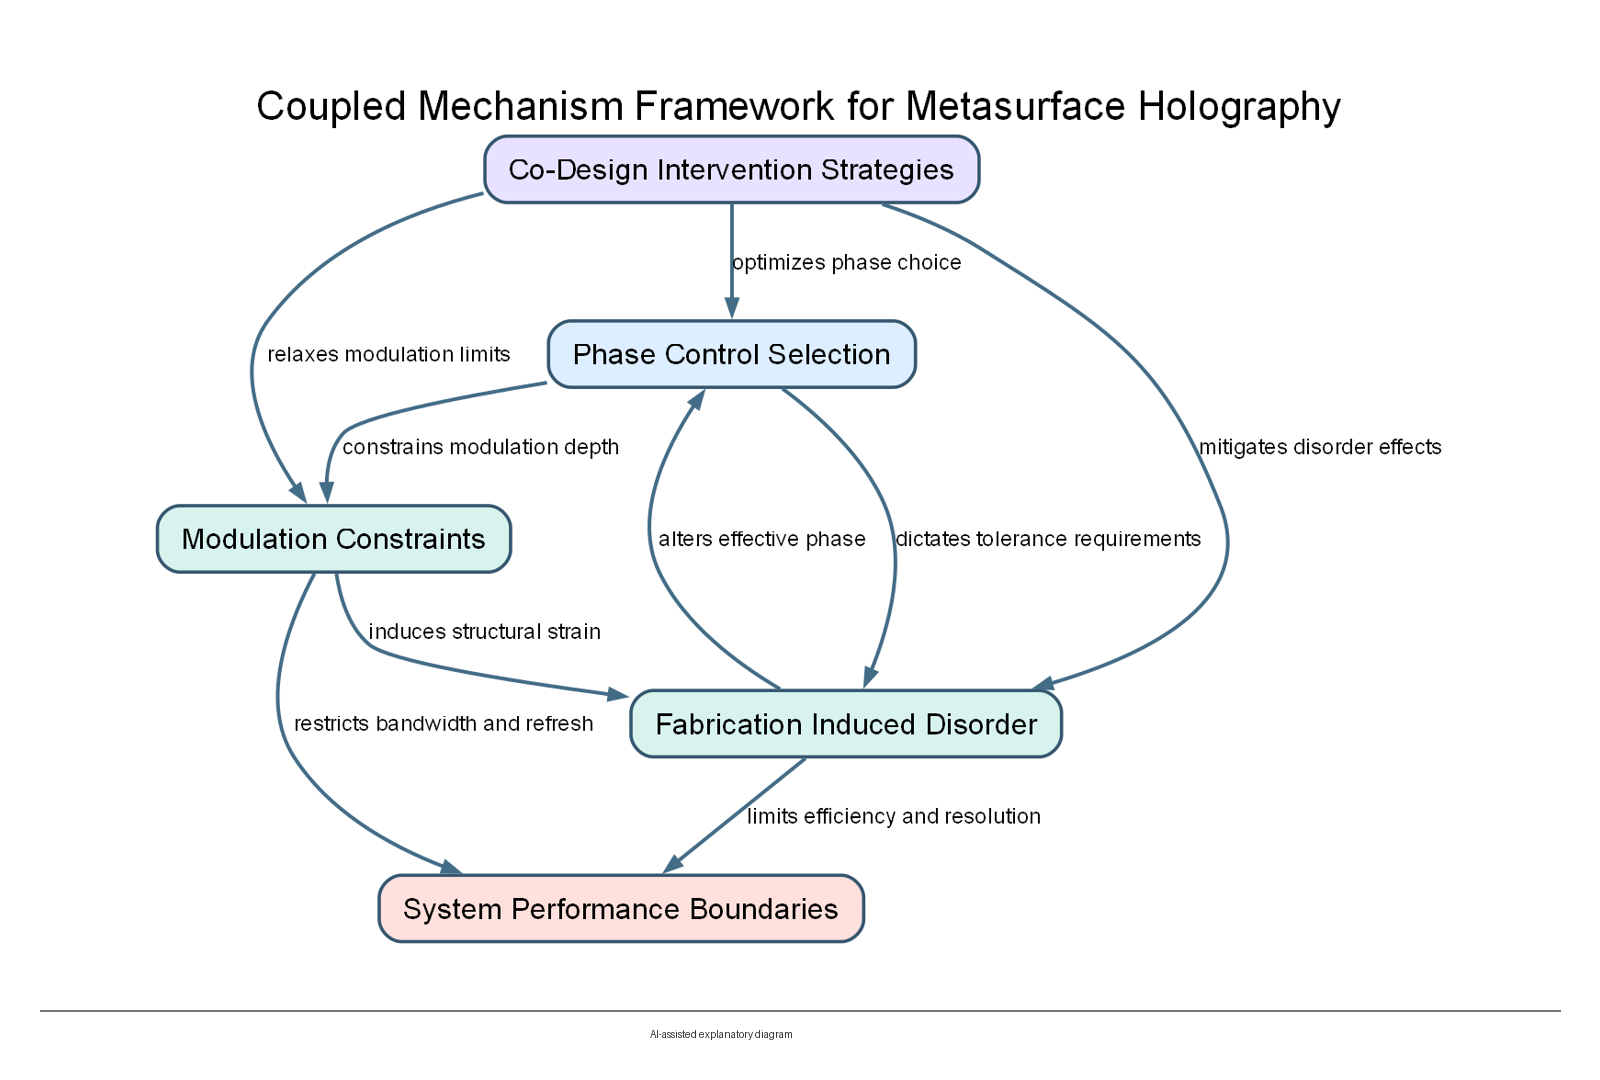
\includegraphics[width=0.9\linewidth,height=\textheight,keepaspectratio,alt={Coupled Mechanism Framework for Metasurface Holography. System performance boundaries emerge from synergistic couplings between phase selection, fabrication disorder, and modulation constraints, necessitating co-design interventions. AI-assisted explanatory diagram; not empirical evidence.}]{figures/03_FIG-GEN-003.png}
\caption{Coupled Mechanism Framework for Metasurface Holography. System performance boundaries emerge from synergistic couplings between phase selection, fabrication disorder, and modulation constraints, necessitating co-design interventions. AI-assisted explanatory diagram; not empirical evidence.}\label{fig:visual_03}
\end{figure}

To resolve the non-uniqueness and convergence bottlenecks inherent in metasurface inverse design, advanced deep learning architectures now provide the specific mechanisms required for co-design frameworks central to this section. Tandem neural networks address the ill-posed mapping by training an inverse network to minimize the error of a re-predicted spectrum rather than direct geometric differences, effectively bypassing the one-to-many problem where distinct geometries yield identical optical responses. \citep{doi_10_1063_5_0171437_92a49ec0} \citep{doi_10_1515_nanoph_2021_0434_1357d09e} Generative approaches have further evolved from Generative Adversarial Networks, which often suffer from mode collapse, to physics-informed diffusion models that reverse a gradual noising process to generate diverse meta-atom shapes under rigorous spectral constraints. \citep{doi_10_71465_fapm546_bda368a5} For handling singular point mutations in electromagnetic property mappings, deep residual networks combined with property classification have demonstrated the ability to predict geometries with mean square errors below 0.23, stabilizing the design of holographic imaging metasurfaces. At the foundation model scale, frameworks like MOCLIP leverage massive experimental datasets of over 466,000 geometry-spectra pairs to learn a shared latent space, enabling zero-shot prediction speeds of approximately 200,000 spectra per second while incorporating fabrication tolerances missing from purely simulated data. Complementing these data-driven strategies, the Adjoint Variable Method (AVM) offers a gradient-based optimization framework that efficiently acquires sensitivity information for complex geometries, accelerating the search for optimal designs without relying solely on large training corpora. \citep{doi_10_2528_pier12020501_bb5007b1} \citep{doi_10_1109_nemo62710_2025_11215427_067e96bb} Together, these architectures shift the paradigm from slow, heuristic fine-tuning to rapid, joint optimization of geometry and spectral response, directly addressing the coupled mechanism bottleneck by ensuring that computational speed does not come at the expense of physical validity or manufacturability. \citep{doi_10_1038_s41467_026_76714_x_8ca5d39b} \citep{doi_10_71465_fapm546_bda368a5} \citep{doi_10_1109_iccem60619_2024_10559188_c3199408} \citep{doi_10_1109_pn62551_2024_10621761_0bc70b78}

The fundamental optimization paradigm dictates the balance between convergence speed and global optimality in navigating high-dimensional, nonconvex design spaces. Inverse design methodologies are currently bifurcating into gradient-based approaches, such as adjoint topology optimization, and gradient-free nature-inspired algorithms. Gradient-based methods leverage the reciprocity theorem to compute the variation of a figure of merit with respect to design parameters, allowing for the simultaneous update of the entire design vector to rapidly reach a local optimum; however, this strategy inherently enforces a local search nature that risks trapping the solution in sub-optimal minima. Conversely, gradient-free techniques, often inspired by natural phenomena like wolf hunting packs, integrate distinct exploration and exploitation phases to escape these local traps without requiring explicit gradient information, yet they frequently suffer from higher computational costs. Traditional heuristic methods like genetic algorithms and particle swarm optimization further illustrate this bottleneck, as they are computationally intensive and non-differentiable, hindering their end-to-end integration with downstream tasks compared to modern differentiable surrogates. This dichotomy reveals that while gradient-based methods offer efficiency for tailored optical functions, they struggle to guarantee global optimality in complex phase landscapes, whereas gradient-free methods offer broader search capabilities at the expense of speed, underscoring the need for strategies that resolve these coupled mechanism bottlenecks. \citep{s2_2516273dc5b4511c838bf9236a61f71f4e32f6b5_1724698f} \citep{doi_10_1088_1367_2630_acfcd6_32444f17} \citep{s2_76a83ea3baed75ad88b7f0782eb9a694a330c853_cee16cac}

Optimization paradigms navigating high-dimensional spaces encounter a fundamental `coupled mechanism bottleneck' where geometric and propagation phases are inextricably linked through shared structural parameters. In dual-spin and frequency-multiplexed metasurfaces, for instance, the phase response at one frequency may depend on a specific subset of nanograting dimensions and orientation angles, while the response at another frequency is determined by the full set of these same variables. \citep{doi_10_1117_1_apn_2_1_016010_57069347} \citep{doi_10_1002_advs_202504634_52bafb6c} This interdependence creates a complex optimization landscape where adjusting a parameter to satisfy one channel inadvertently alters the response of another, introducing significant cross-talk. Current inverse design approaches often attempt to resolve this by treating the metasurface as an isolated component, utilizing classifiers and iterative neural networks to suppress specific phase cross-talks based on preset conditions. However, such methods frequently fail to account for broader system-level interactions, such as coupling between adjacent meta-atoms or substrate effects, because they rely on loss functions that fit target oscillatory behaviors without fully embedding the physical constraints of the entire optical environment. Consequently, treating the device in isolation limits the predictive accuracy of simulation-to-experiment workflows, reinforcing the chapter's thesis that resolving these trade-offs requires moving beyond component-level optimization toward integrated co-design frameworks. \citep{doi_10_1117_1_apn_2_1_016010_57069347} \citep{doi_10_1515_nanoph_2020_0379_1cc596ab}

Co-design frameworks have emerged as a primary strategy to resolve the coupled mechanism bottleneck identified previously, defined here as joint optimization protocols that integrate computational inverse design directly with fabrication-aware constraints. The intuitive premise is that high-fidelity phase control cannot be achieved in isolation from the physical realities of manufacturing disorder; instead, these tolerances must be embedded within the optimization loop itself. Mechanistically, this is realized by constructing combined loss functions or unified machine-learning architectures that account for non-uniqueness and oscillatory behaviors inherent to resonant components. For instance, recent approaches utilize classifiers to distinguish specific cross-talk conditions between geometric and propagation phases, allowing adaptive optimization of meta-atom parameters to satisfy multi-channel wavefront tailoring requirements. Similarly, unified frameworks address incomplete design specifications by mapping feature vectors through conditional decoders while employing pre-trained forward models to mitigate non-uniqueness effects that typically deteriorate convergence. These methods demonstrate significant efficiency gains, reducing design time compared to traditional genetic algorithms while maintaining robustness across expanded parameter ranges. However, while such strategies effectively bridge the gap between idealized simulation and experimental feasibility, consensus on optimal joint optimization protocols remains incomplete, highlighting the need for the broader system-level integration discussed next. \citep{doi_10_1117_1_apn_2_1_016010_57069347} \citep{doi_10_1515_nanoph_2020_0379_1cc596ab} \citep{doi_10_23919_piers_fall62445_2025_11394631_4fdb8517}

Co-design must further expand to end-to-end system optimization, where metasurface geometry and downstream computational algorithms are jointly tuned to overcome physical limitations. In this framework, the optical element does not need to form a perfect image independently; instead, it encodes information in a way that a specific post-processing algorithm can optimally reconstruct. For instance, recent work demonstrates that co-optimizing a single-layer metasurface with a nonlinear Planck-regression algorithm enables high-quality temperature map reconstruction from long-wave infrared radiation, effectively bypassing the delay-bandwidth constraints that typically require bulky multi-layer optics. This joint design relies on differentiable electromagnetic simulators that link geometric parameters directly to complex reflection and transmission coefficients, accurately accounting for multiple internal reflections within thin-film layers during the optimization process. Furthermore, hybrid meta-optical systems combine these flat elements with conventional refractive lenses to leverage the strengths of both platforms: refractive components provide bulk optical power while metasurfaces correct aberrations, achieving large spatial-spectral bandwidths suitable for augmented reality thermal imaging. By treating the sensor, optics, and algorithm as a unified differentiable pipeline, these strategies resolve trade-offs between miniaturization and performance that plague independently optimized subsystems, directly addressing the chapter's thesis that breaking the coupled mechanism bottleneck requires holistic design frameworks. \citep{doi_10_1002_adom_202402498_4083d234} \citep{doi_10_1002_lpor_71431_d57da40c}

Emerging physical principles offer a pathway to fundamentally break performance limits through high-quality resonances, complementing system-level co-design that addresses architectural trade-offs. Symmetry-protected bound states in the continuum (BICs) represent modes that are theoretically decoupled from free space; by introducing controlled symmetry-breaking perturbations, such as dimerization, these evolve into leaky quasi-BICs with tunable quality factors (Q-factors) that scale inversely with perturbation strength. This mechanism enables precise wavefront control while maintaining strong field confinement, as demonstrated by toroidal-dipole-driven metasurfaces that achieve complete polarization selectivity and stable operation under wide-angle oblique incidence, outperforming prior designs limited to normal incidence. Toroidal-dipole-driven quasi-bound states in the continuum have been utilized to enable wide-angle near-field image display in dielectric metasurfaces, achieving complete polarization selectivity and stable operation under oblique incidence. \citep{s2_5a46bf1115a13c8e88d03d52a56e80871e3550cd_094f009d} Complementing these physical advances, computational frontiers employing frequency transfer techniques based on Euler latent dynamics propose methods to co-optimize metasurfaces under complex multi-physics coupling constraints. Together, these developments suggest that resolving the coupled mechanism bottleneck requires not only integrating fabrication tolerances but also leveraging exotic resonant states and advanced inverse design algorithms to jointly optimize optical efficiency, angular robustness, and system functionality. \citep{doi_10_1103_physrevapplied_21_044004_d1b93ffe} \citep{s2_5a46bf1115a13c8e88d03d52a56e80871e3550cd_094f009d} \citep{doi_10_1038_s41467_025_57516_z_7c69e056}

\section{Conclusion}\label{conclusion}

This review has systematically mapped the technological pipeline of metasurface-based holography, tracing the trajectory from fundamental phase control mechanisms to complex system-level applications. The central finding emerging from this analysis is that while computational inverse design has effectively unlocked theoretically unlimited design spaces, the practical realization of high-fidelity, dynamic holographic systems remains constrained by a persistent ``design-reality gap.'' This gap is a matter of incremental engineering improvement and stems from the uncoupled treatment of physical mechanisms, fabrication tolerances, and system integration throughout the current development lifecycle.

Metasurface holography relies on three distinct phase control mechanisms---geometric, propagation, and hybrid approaches---each imposing intrinsic trade-offs among efficiency, bandwidth, and polarization sensitivity. As established, geometric phase offers robust polarization control but suffers from chromatic limitations, while propagation phase provides high efficiency at the cost of narrow bandwidth due to resonant dispersion. Although hybrid strategies attempt to navigate these physical boundaries, they introduce new complexities in design non-uniqueness. To address these challenges, ODNN research has transitioned from intuition-based heuristics to sophisticated computational inverse design frameworks, including deep learning surrogates and adjoint-based topology optimization. These algorithms successfully map desired electromagnetic responses to nanostructure geometries, overcoming the ill-posed nature of the inverse scattering problem. However, these computational successes often rely on idealized models that assume perfect geometric control, ignoring the stochastic realities of nanofabrication.

This reliance on idealization creates a critical bottleneck when transitioning to physical realization. The review highlights that current nanofabrication processes, particularly serial writing techniques like electron-beam lithography, impose strict tolerance thresholds that systematically degrade holographic fidelity below theoretical predictions. While scalable methods such as nanoimprint lithography offer a pathway to mass production, there is a notable deficit in experimental validation for maintaining nanometer-scale fidelity over meter-scale areas. Consequently, the sophisticated freeform patterns generated by inverse design algorithms frequently encounter a ``fabrication ceiling,'' where the very geometric diversity that enables complex wavefront control becomes a source of uncertainty and performance loss in physical devices.

Furthermore, the extension of metasurfaces into dynamic applications reveals a fundamental ``speed-efficiency-bandwidth trilemma.'' Active modulation mechanisms, ranging from phase-change materials and liquid crystals to MEMS actuators, enable real-time reconfiguration but invariably introduce penalties in diffraction efficiency, spectral range, or switching speed. No single platform currently dominates all three axes, forcing designers to accept specific compromises based on application requirements. This trade-off is exacerbated in display and imaging architectures, where the distinction between human-perception metrics (brightness, refresh rate) and machine-performance metrics (resolution, signal-to-noise ratio) necessitates tailored integration strategies. The recurrence of detailed algorithmic descriptions in application-specific sections underscores a systemic issue: the tendency to re-optimize design parameters in isolation rather than leveraging unified, physics-informed frameworks.

In conclusion, the primary barrier to the commercial readiness of metasurface holography is no longer the lack of computational tools to generate complex designs, but the failure to integrate these tools with the constraints of manufacturing and system-level operation. The path forward demands a paradigm shift from component-level optimization to holistic co-design. Future advancements will likely depend on frameworks that jointly optimize meta-atom geometry, fabrication-induced disorder, and downstream computational reconstruction algorithms. By embedding physical realizability and system-level metrics directly into the inverse design loop, researchers can bridge the gap between simulated optimality and experimental reality, ultimately enabling the robust, scalable, and dynamic holographic systems envisioned by ODNN research's theoretical foundations.

\bibliographystyle{unsrtnat}
\bibliography{references}
\end{document}
